% ============================================================
%  NEORV32 Accelerator for Cryptography
%  Ascon-AEAD128 Hardware Accelerator
%  Project Report
%  Author: Mohammadi Masoudi Ramin
% ============================================================
\documentclass[11pt,a4paper]{article}

\usepackage[T1]{fontenc}
\usepackage[utf8]{inputenc}
\usepackage[margin=2.5cm]{geometry}
\usepackage{hyperref}
\usepackage{booktabs}
\usepackage{longtable}
\usepackage{array}
\usepackage{xcolor}
\usepackage{colortbl}
\usepackage{listings}
\usepackage{tikz}
\usetikzlibrary{arrows.meta,positioning,shapes.geometric,calc,fit}
\usepackage{pgfplots}
\pgfplotsset{compat=1.16}
\usepackage{amsmath}
\usepackage{amssymb}
\usepackage{graphicx}
\usepackage{fancyhdr}
\usepackage{titlesec}
\usepackage{enumitem}
\usepackage{float}
\usepackage{multirow}
\usepackage{tabularx}
\usepackage{tcolorbox}
\tcbuselibrary{skins,breakable}

\definecolor{docblue}{RGB}{0,51,102}
\definecolor{doclblue}{RGB}{0,85,128}
\definecolor{reqbg}{RGB}{235,244,255}
\definecolor{reqframe}{RGB}{70,100,150}
\definecolor{nfrbg}{RGB}{240,255,240}
\definecolor{nfrframe}{RGB}{40,120,70}
\definecolor{codebg}{RGB}{247,247,247}
\definecolor{tabhead}{RGB}{0,51,102}
\definecolor{rowalt}{RGB}{243,247,255}
\definecolor{warnbg}{RGB}{255,251,230}
\definecolor{warnframe}{RGB}{170,120,0}
\definecolor{okgreen}{RGB}{40,120,70}
\definecolor{barhw}{RGB}{0,85,128}
\definecolor{barsw}{RGB}{170,120,0}

\hypersetup{
  colorlinks=true, linkcolor=docblue, urlcolor=doclblue, citecolor=docblue,
  pdftitle={NEORV32 Ascon-AEAD128 Hardware Accelerator: Project Report},
  pdfauthor={Mohammadi Masoudi Ramin}
}

\titleformat{\section}
  {\Large\bfseries\color{docblue}}{\thesection}{1em}{}
  [\color{docblue}\rule{\linewidth}{0.6pt}]
\titleformat{\subsection}
  {\large\bfseries\color{docblue}}{\thesubsection}{1em}{}
\titleformat{\subsubsection}
  {\normalsize\bfseries\color{doclblue}}{\thesubsubsection}{1em}{}

\pagestyle{fancy}\fancyhf{}
\fancyhead[L]{\small\color{docblue}\textbf{NEORV32 Ascon-AEAD128 Hardware Accelerator}}
\fancyhead[R]{\small\color{docblue}Project Report}
\fancyfoot[C]{\small\thepage}
\renewcommand{\headrulewidth}{0.4pt}

\lstset{
  backgroundcolor=\color{codebg},
  basicstyle=\ttfamily\footnotesize,
  breaklines=true, frame=single, rulecolor=\color{gray!35},
  numbers=none,
  keywordstyle=\color{docblue}\bfseries,
  commentstyle=\color{gray!65}\itshape,
  stringstyle=\color{doclblue},
  xleftmargin=1em, aboveskip=8pt, belowskip=6pt
}

\newcommand{\warn}[1]{%
  \begin{tcolorbox}[enhanced, colback=warnbg, colframe=warnframe,
    arc=2pt, boxrule=0.5pt, left=6pt, right=6pt, top=3pt, bottom=3pt,
    before upper={\small}]
  \textbf{\color{warnframe}Honest caveat:} #1
  \end{tcolorbox}\vspace{3pt}}

\newtcolorbox{bugbox}[1]{
  enhanced, breakable, colback=reqbg, colframe=reqframe,
  arc=2pt, boxrule=0.5pt, left=6pt, right=6pt, top=3pt, bottom=3pt,
  attach boxed title to top left={yshift=-2mm, xshift=8pt},
  boxed title style={colback=reqframe, arc=2pt, boxrule=0pt,
                     left=4pt, right=4pt, top=2pt, bottom=2pt},
  title={\small\bfseries\color{white}#1}, before upper={\small}}

\newcolumntype{L}[1]{>{\raggedright\arraybackslash}p{#1}}
\newcolumntype{C}[1]{>{\centering\arraybackslash}p{#1}}
\newcommand{\thd}[1]{\cellcolor{tabhead}\color{white}\textbf{\small #1}}
\newcommand{\trow}{\rowcolor{rowalt}}
\newcommand{\code}[1]{\texttt{\small #1}}
\newcommand{\ok}{\textbf{\color{okgreen}\checkmark}}

\setlength{\parskip}{5pt}
\setlength{\parindent}{0pt}
\setlist[itemize]{noitemsep, topsep=2pt}
\setlist[enumerate]{noitemsep, topsep=2pt}

% ============================================================
\begin{document}
% ============================================================

\begin{titlepage}
\centering
\vspace*{2.5cm}
{\color{docblue}\rule{\linewidth}{1.2pt}}\\[0.6cm]
{\Huge\bfseries\color{docblue} NEORV32 Ascon-AEAD128\\[0.2cm] Hardware Accelerator}\\[0.4cm]
{\LARGE\color{doclblue} Project Report}\\[0.3cm]
{\color{docblue}\rule{\linewidth}{1.2pt}}\\[1.2cm]
{\large Results, methodology, and engineering challenges of an\\
open-source Ascon accelerator validated on silicon.}\\[1.6cm]
\begin{tcolorbox}[width=0.8\linewidth, colback=nfrbg, colframe=nfrframe,
  halign=center, arc=3pt]
{\large\bfseries\color{nfrframe} Headline result}\\[2pt]
All 8 test cases correct on hardware; the accelerator is\\
\textbf{$\sim$18$\times$ to $\sim$57$\times$ faster} than the software reference\\
on the same RISC-V core.
\end{tcolorbox}
\par\vspace{1.6cm}
{\large\textbf{Mohammadi Masoudi Ramin}}\\[0.3cm]
{\normalsize Politecnico di Milano}\\
\vfill
\end{titlepage}

\tableofcontents
\newpage

% ------------------------------------------------------------
\section{Executive Summary}
This project designed, verified, and validated on silicon a hardware accelerator
for Ascon-AEAD128, the NIST lightweight authenticated-encryption standard
(SP~800-232). The accelerator was generated from a typed Python golden model,
integrated as an external-bus peripheral on a fully-open NEORV32 RISC-V
system-on-chip, built end-to-end with an all-open toolchain (GHDL, Yosys,
nextpnr, Apicula), and programmed onto a Tang Nano 20K FPGA board.

On hardware, an on-chip benchmark encrypted and decrypted eight
associated-data/plaintext combinations and checked every result against a
software reference running on the same CPU. \textbf{All eight cases were correct},
and the hardware was between \textbf{17.6$\times$ and 57.4$\times$ faster} than the
reference software, depending on payload size. The remainder of this report
explains what was measured, how, the engineering challenges overcome, the design
choices behind them, and an honest account of what the numbers do and do not
claim.

% ------------------------------------------------------------
\section{Objectives and Method}

\subsection{Objectives}
\begin{enumerate}
\item Implement Ascon-AEAD128 in hardware, provably matching the standard.
\item Make it usable from software through a clean C interface on a RISC-V CPU.
\item Build the whole system with open-source tools only, reproducibly.
\item Validate on real silicon and quantify the speed-up over software.
\end{enumerate}

\subsection{Method}
The accelerator was generated from a golden model that passes the NIST
Known-Answer Tests, then verified in four layers (model $\to$ RTL $\to$ driver
$\to$ end-to-end co-simulation; 119 automated tests). It was integrated on
NEORV32, synthesised with the open flow, and flashed to the board. On-chip, a
benchmark timed a software Ascon reference and the hardware accelerator on the
same inputs, verified equality, and reported cycle counts. The architecture and
verification are detailed in the companion Design Document; this report
concentrates on the outcome.

% ------------------------------------------------------------
\section{The Test Platform}
\renewcommand{\arraystretch}{1.25}
\begin{center}
\begin{tabular}{L{4.8cm} L{9.4cm}}
\thd{Component} & \thd{Configuration}\\
\trow FPGA board & Sipeed Tang Nano 20K\\
FPGA device & Gowin GW2AR-18 (GW2A-18C family)\\
\trow Soft CPU & NEORV32, \code{rv32i} + Zicntr, no M extension\\
Clock & 27\,MHz (board oscillator; timing closed with $\sim$2$\times$ margin)\\
\trow Memory & IMEM 16\,KB, DMEM 8\,KB (on-chip block RAM)\\
Accelerator bus & Wishbone-b4 on NEORV32 XBUS, base \code{0x9000\,0000}\\
\trow Toolchain & GHDL $\to$ Yosys $\to$ nextpnr-himbaechel $\to$ Apicula (all open)\\
Firmware toolchain & RISC-V GCC, freestanding, soft-float\\
\end{tabular}
\end{center}
\renewcommand{\arraystretch}{1}

% ------------------------------------------------------------
\section{Results}

\subsection{Correctness}
Across all eight cases, hardware encryption produced ciphertext and tag identical
to the software reference; hardware decryption recovered the plaintext with a
valid tag; and (in the standalone self-test) a tampered ciphertext was correctly
rejected. Every \code{enc\_ok}, \code{dec\_ok}, and \code{tag\_valid} flag was
set. The on-chip verdict was \textbf{PASS} on all eight of eight cases.

\subsection{Performance}
The measured cycle counts and resulting speed-ups (from the on-chip benchmark):

\renewcommand{\arraystretch}{1.25}
\begin{center}
{\small\setlength{\tabcolsep}{3.8pt}
\begin{tabular}{L{2.2cm} C{0.8cm} C{0.8cm} r r C{1.15cm} r r C{1.15cm} C{0.7cm}}
\thd{Case} & \thd{AD} & \thd{PT} & \thd{SW enc} & \thd{HW enc} & \thd{Enc$\times$}
          & \thd{SW dec} & \thd{HW dec} & \thd{Dec$\times$} & \thd{OK}\\
\trow \code{empty}     & 0  & 0  & 38\,866 & 684   & \textbf{56.8} & 39\,241 & 684   & \textbf{57.4} & \ok\\
\code{ad8}             & 8  & 0  & 50\,205 & 1\,335 & 37.6 & 50\,579 & 1\,335 & 37.9 & \ok\\
\trow \code{pt8}       & 0  & 8  & 39\,458 & 1\,239 & 31.9 & 39\,665 & 1\,239 & 32.0 & \ok\\
\code{ad8\_pt8}        & 8  & 8  & 50\,797 & 1\,890 & 26.9 & 51\,003 & 1\,890 & 27.0 & \ok\\
\trow \code{pt16}      & 0  & 16 & 52\,156 & 2\,007 & 26.0 & 52\,595 & 2\,007 & 26.2 & \ok\\
\code{pt24}            & 0  & 24 & 52\,748 & 2\,763 & 19.1 & 53\,019 & 2\,763 & 19.2 & \ok\\
\trow \code{pt32}      & 0  & 32 & 65\,447 & 3\,531 & 18.5 & 65\,950 & 3\,531 & 18.7 & \ok\\
\code{ad16\_pt32}      & 16 & 32 & 86\,984 & 4\,948 & 17.6 & 87\,486 & 4\,948 & 17.7 & \ok\\
\end{tabular}}
\end{center}
\renewcommand{\arraystretch}{1}
{\small AD and PT are associated-data and plaintext bytes. SW/HW columns are clock
cycles at 27\,MHz. Speed-up is SW\,$\div$\,HW.}

\subsection{Cycle counts, visualised}
\begin{center}
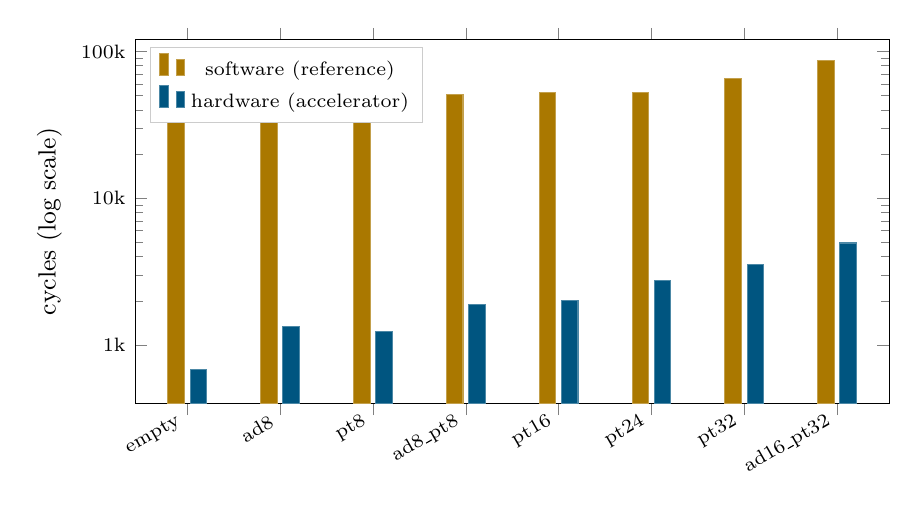
\begin{tikzpicture}
\begin{axis}[
  width=0.92\linewidth, height=6.2cm,
  ybar, bar width=6pt,
  ymode=log, log origin=infty,
  ymin=400, ymax=120000,
  ylabel={\small cycles (log scale)},
  symbolic x coords={empty,ad8,pt8,ad8\_pt8,pt16,pt24,pt32,ad16\_pt32},
  xtick=data, x tick label style={rotate=30, anchor=east, font=\scriptsize},
  ytick={1000,10000,100000},
  yticklabels={1k,10k,100k},
  legend style={at={(0.02,0.98)}, anchor=north west, font=\scriptsize, draw=gray!40},
  enlarge x limits=0.08, tick label style={font=\scriptsize}]
\addplot[fill=barsw, draw=barsw!70] coordinates {
  (empty,38866)(ad8,50205)(pt8,39458)(ad8\_pt8,50797)(pt16,52156)(pt24,52748)(pt32,65447)(ad16\_pt32,86984)};
\addplot[fill=barhw, draw=barhw!70] coordinates {
  (empty,684)(ad8,1335)(pt8,1239)(ad8\_pt8,1890)(pt16,2007)(pt24,2763)(pt32,3531)(ad16\_pt32,4948)};
\legend{software (reference), hardware (accelerator)}
\end{axis}
\end{tikzpicture}
\end{center}

\subsection{Speed-up trend}
\begin{center}
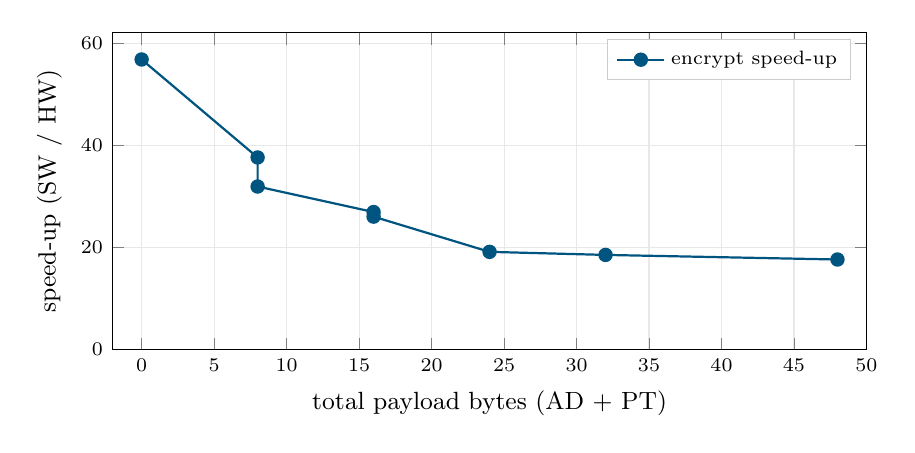
\begin{tikzpicture}
\begin{axis}[
  width=0.92\linewidth, height=5.6cm,
  ylabel={\small speed-up (SW / HW)},
  xlabel={\small total payload bytes (AD + PT)},
  ymin=0, ymax=62,
  xmin=-2, xmax=50,
  grid=both, grid style={gray!18},
  mark size=2.2pt, tick label style={font=\scriptsize},
  legend style={at={(0.98,0.98)}, anchor=north east, font=\scriptsize, draw=gray!40}]
% x = AD+PT total bytes, y = encrypt speedup
\addplot[color=barhw, thick, mark=*] coordinates {
  (0,56.8)(8,37.6)(8,31.9)(16,26.9)(16,26.0)(24,19.1)(32,18.5)(48,17.6)};
\legend{encrypt speed-up}
\end{axis}
\end{tikzpicture}
\end{center}

The speed-up is largest for tiny payloads and falls as payloads grow. This is the
expected shape and is explained by \emph{where the hardware spends its cycles}:
the hardware figure includes the time the CPU takes to move data in and out of the
accelerator word-by-word over the memory-mapped interface, and that data-movement
cost grows with payload size while the fixed cryptographic cost does not.

% ------------------------------------------------------------
\section{What the Speed-up Is Measured Against}
Being precise here matters, because ``57$\times$ faster'' is meaningless without
saying faster \emph{than what}.

\begin{itemize}
\item \textbf{Software (numerator):} CPU clock cycles, read with \code{rdcycle},
      around a clean 64-bit C reference implementation of Ascon-AEAD128 (the
      straightforward NIST-style code), running on the same NEORV32 core (a
      32-bit \code{rv32i} CPU at 27\,MHz). Because the core is 32-bit, each 64-bit
      Ascon word costs several instructions.
\item \textbf{Hardware (denominator):} the accelerator's own cycle-counter
      register, i.e.\ the number of clock cycles it was busy for the operation,
      at the same 27\,MHz.
\end{itemize}

So the honest phrasing is: \emph{the hardware crypto engine versus a reference
software Ascon on the same SoC}. It is a fair, same-platform, same-clock
comparison.

\warn{The software baseline is a \emph{reference}, not a hand-optimised or
assembly implementation --- an optimised software Ascon on the same core would be
faster, narrowing the gap (though hardware would still win). And the hardware
counter measures the operation from start to done, so it \emph{excludes} the
register-setup writes before and the tag/output reads after. A fully end-to-end
wall-clock comparison (CPU cycles around the entire driver call) would show
somewhat lower speed-ups, most noticeably for the tiny \code{empty} case. The
$\sim$18$\times$ on real payloads is closer to the end-to-end story than the
$\sim$57$\times$ on the empty one.}

% ------------------------------------------------------------
\section{Engineering Challenges}
The path from ``simulation passes'' to ``correct on silicon'' surfaced a sequence
of real bugs. Each was diagnosed from concrete evidence --- a linker error, a
processor panic with a fault address, a serial trace --- rather than guesswork.
They are worth recording, because they are exactly the class of problem a
simulation-only flow does not reveal.

\begin{bugbox}{1 --- Read-only build environment}
The NEORV32 build compiled a host helper tool and memory images \emph{into} its
own source tree, which on this setup lives in the read-only Nix store. Fixed by
redirecting all generated artefacts into a writable build directory while still
reading sources from the store.
\end{bugbox}

\begin{bugbox}{2 --- Toolchain name mismatch}
The firmware Makefile expected a compiler named \code{riscv-none-elf-gcc}, but the
pinned toolchain provided \code{riscv32-none-elf-gcc}. Fixed by auto-detecting
whichever RISC-V compiler is on the path.
\end{bugbox}

\begin{bugbox}{3 --- Float-ABI mismatch}
The standard library in the toolchain was compiled double-float, but the CPU has
no FPU and the firmware is soft-float; they refuse to link. Resolved with a
freestanding build that supplies its own soft-float 64-bit helpers instead of the
incompatible library.
\end{bugbox}

\begin{bugbox}{4 --- Stack past the end of memory (silent trap)}
The firmware was linked assuming 16\,KB of data RAM, but the SoC provides 8\,KB.
The startup code placed the stack pointer 8\,KB beyond real memory, so the very
first stack write trapped --- before the program could print anything. The symptom
was a boot with no output. Fixed by matching the firmware's memory sizes to the
hardware.
\end{bugbox}

\begin{bugbox}{5 --- Flaky debugger and shifting serial ports}
The board's USB debugger periodically re-enumerated, swapping the serial device
names and occasionally wedging so that programming itself failed. Handled by
addressing the UART through its stable by-identifier path and power-cycling to
recover the debugger.
\end{bugbox}

\begin{bugbox}{6 --- The bus handshake (the key hardware bug)}
NEORV32's external bus drives its strobe as a \emph{single-cycle pulse} and only
samples the acknowledge in the cycle \emph{after} the strobe. The first version of
the Wishbone adapter asserted its acknowledge \emph{during} the strobe --- the one
cycle the CPU was not looking. The CPU never saw it, waited out its bus timeout,
and raised a store-access fault at the accelerator's address. Fixed with a
handshake state machine that latches the strobe and acknowledges in the following
cycle; then re-verified in simulation against a bus master that reproduces
NEORV32's exact timing.
\end{bugbox}

\begin{bugbox}{7 --- Fitting the FPGA}
With the accelerator added, place-and-route reported the design at the device's
utilisation limit and could not find a legal placement. The CPU's hardware
multiply/divide unit was the largest removable block and is unused by the
\code{rv32i} firmware, so dropping it freed enough logic to fit --- with the
firmware providing software multiply/divide.
\end{bugbox}

\begin{bugbox}{8 --- Protocol ordering (the last bug)}
The driver wrote the \code{START} command \emph{after} streaming the payload for
the memory-mapped data plane, but the accelerator is a start-first stream engine:
it only accepts data after being started. Streaming first hit the idle engine,
stalled the streaming write, and timed out --- again a fault at the data-in
register. Fixed by writing \code{START} \emph{before} streaming, matching the
engine and the simulation.
\end{bugbox}

\subsection{The pattern that mattered}
Bugs 6 and 8 were the two standing between ``the CPU cannot reach the
accelerator'' and the clean result. Both were found the same way: the processor
panicked with a precise fault address (\code{0x9000\,0000} for a control write,
\code{0x9000\,0044} for a data-in write), and that address named exactly which
register --- and therefore which mechanism --- had failed. Instrumenting the
firmware with breadcrumb prints, and a minimal ``hello'' program to isolate the
runtime from the accelerator, turned each silent hang into a located fault.

% ------------------------------------------------------------
\section{Design Choices and Their Consequences}
\renewcommand{\arraystretch}{1.3}
\begin{center}
\begin{tabular}{L{4.4cm} L{9.2cm}}
\thd{Choice} & \thd{Consequence}\\
\trow Golden-model-first generation & RTL and reference share one definition;
    the verification oracle is free. Bugs were interface bugs, never crypto bugs.\\
1 round / cycle permutation & Smallest core; fit the small FPGA. Crypto latency is
    a handful of cycles --- not the bottleneck.\\
\trow Memory-mapped word data plane & Simple, no DMA. But it makes CPU
    data-movement the dominant cost for large payloads --- the reason speed-up
    falls with size.\\
XBUS peripheral, not an instruction & Loose coupling, no pipeline changes ---
    but every access is a bus transaction with the CPU in the loop.\\
\trow Drop the M extension & Freed the logic to fit. Safe because the firmware is
    \code{rv32i} and the bootloader needs no multiply.\\
Fully-open Nix toolchain & Reproducible and vendor-free --- at the cost of the
    bleeding-edge sharp edges that became challenges 1--3.\\
\end{tabular}
\end{center}
\renewcommand{\arraystretch}{1}

% ------------------------------------------------------------
\section{Limitations and Future Work}
\begin{itemize}
\item \textbf{Payload bound.} 32 bytes of associated data and 32 of message per
      call. Rate-block streaming for arbitrary lengths is the clear next feature
      and is a natural extension of the generator.
\item \textbf{Data-movement bottleneck.} A DMA path or a wider bus datapath would
      raise the large-payload numbers, which are currently limited by the
      word-at-a-time interface, not by the crypto.
\item \textbf{Mode coverage.} Only AEAD128 runs on hardware; hash/XOF modes exist
      in the model and could be integrated.
\item \textbf{Fair end-to-end metric.} Adding a second measurement that wraps the
      CPU cycle counter around the entire driver call would report the full
      wall-clock speed-up, not just the accelerator's busy time.
\item \textbf{Security characterisation.} No constant-time or side-channel
      analysis has been done; this is a functional and performance result.
\end{itemize}

% ------------------------------------------------------------
\section{Conclusion}
The project achieved its objectives: a standard-conformant Ascon-AEAD128
accelerator, generated from a verified model, usable from C on a RISC-V SoC, built
entirely with open tools, and \emph{validated on silicon} with every test case
correct and a measured 18--57$\times$ speed-up over reference software on the same
core. Equally valuable is the honest engineering record --- eight distinct bugs,
each diagnosed from the board's own evidence, spanning the build environment, the
toolchain, memory layout, the bus handshake, device fit, and the driver protocol.
The two that mattered most, the pulsed-strobe bus handshake and the start-first
protocol order, are precisely the kind of hardware/software boundary issue that
only a real, end-to-end validation exposes.

\vfill
\begin{center}\small\color{gray}
Project Report --- companion to the RASD and the Design Document.
\end{center}

\end{document}
